%% Submissions for peer-review must enable line-numbering
%% using the lineno option in the \documentclass command.
%%
%% Preprints and camera-ready submissions do not need
%% line numbers, and should have this option removed.
%%
%% Please note that the line numbering option requires
%% version 1.1 or newer of the wlpeerj.cls file, and
%% the corresponding author info requires v1.2

% \documentclass[fleqn,10pt, lineno]{wlpeerj} % for journal submissions
\documentclass[fleqn,10pt]{wlpeerj} % for preprint submissions
\usepackage{textcomp} %for \textgreater
\usepackage{wasysym} %for \times
\usepackage{hyperref}

\title{Patterned progression of gut microbiota in association with preterm infants to necrotizing enterocolitis and late onset sepsis: prospective pilot data from a non-Western population}

\author[1]{Jiayi Liu}
\author[2]{Jianhua Sun}
\author[3]{Yuqing Li}
\author[4]{Yi Feng}
\author[5]{Liya Pan}
\author[6]{Zhoulonglong Xie}
\author[7]{Zhilong Yan}
\author[8]{Jianhua Zhao}
\author[9]{Li Hong}


\affil[1]{Department of Clinical Nutrition, Shanghai Children's Medical Center, School of Medicine Shanghai Jiao Tong University, Shanghai, China}
\affil[2]{Department of Clinical Nutrition, Shanghai Children's Medical Center, School of Medicine Shanghai Jiao Tong University, Shanghai, China}
\affil[3]{Department of Clinical Nutrition, Shanghai Children's Medical Center, School of Medicine Shanghai Jiao Tong University, Shanghai, China}
\affil[4]{Department of Clinical Nutrition, Shanghai Children's Medical Center, School of Medicine Shanghai Jiao Tong University, Shanghai, China}
\affil[5]{Department of Clinical Nutrition, Shanghai Children's Medical Center, School of Medicine Shanghai Jiao Tong University, Shanghai, China}
\affil[6]{Department of Clinical Nutrition, Shanghai Children's Medical Center, School of Medicine Shanghai Jiao Tong University, Shanghai, China}
\affil[7]{Department of Clinical Nutrition, Shanghai Children's Medical Center, School of Medicine Shanghai Jiao Tong University, Shanghai, China}
\affil[8]{Shanghai Majorbio Bio-Pharm Technology Co., Ltd, Shanghai, China}
\affil[9]{Department of Clinical Nutrition, Shanghai Children's Medical Center, School of Medicine Shanghai Jiao Tong University, Shanghai, China}
\corrauthor[9]{Li Hong}{hongli@scmc.com.cn}

%\keywords{Gut Microbiota, Preterm Infant, Necrotizing Enterocolitis, Neonatal Late Onset Sepsis, High Throughput DNA Sequencing}

%%%%%%%%%%   abstract  %%%%%%%%%%
\begin{abstract}
  Recent studies have associated necrotizing enterocolitis (NEC) and late-onset sepsis(LOS), two common complications of preterm births, to gut microbiota dysbiosis. Similar studies in Asian population remain scant. In this pilot study, we profiled gut microbiota of four NEC and three LOS patients among 24 preterm Chinese infants starting from birth until decease or discharge. The microbial community diversities in case stools differed significantly from those in control ones. These differences emerged only after the third day of life and persisted throughout the courses of both NEC and LOS. In ZIBR models, higer Bacillus (p = 0.032) and lower Solibacillus (p = 0.047) were associated with both NEC and LOS onset. \textit{Enterococcus}, \textit{Streptococcus} and \textit{Peptoclostridium} were prominent in NEC progression and \textit{Klebsiella} in LOS cases. Consistent (not really...) with studies in European and American countries, these changes in diversity and composition preceded the onset of diseases and might have played an essential role in disease progression. [\emph{Inconsistant with studies in European an American countries, these results should be a starting point for further studying of microbial factors involved in preterm-associated complications specifically within Chinese population...???}] These results warrant further studies to identify correspondent microbial patterns, etiological strains and underlying mechanisms.
%The microbial community structure in case stools differed significantly from those in control stools. These differences emerged only after the fi rst month of age. In mixed models, the time- by-necrotising-enterocolitis interaction was positively associated with Gammaproteobacteria (p=0·0010) and negatively associated with strictly anaerobic bacteria, especially Negativicutes (p=0·0019). We studied 1094 stool samples from 44 infants in the secondary cohorts. 18 infants developed necrotising enterocolitis (cases) and 26 were controls. These associations were strongest in both the primary cohort and the overall cohort for infants born at less than 27 weeks’ gestation.
\end{abstract}

\begin{document}

\flushbottom
\maketitle
\thispagestyle{empty}

%%%%%%%%%%%%%%%%%%%%%%%%% INTRODUCTION %%%%%%%%%%%%%%%%%%%%%%%%%%%
\section*{Introduction}
The gut microbiota is a key contributor to human health. Imbalance of the microbial community, termed dysbiosis, is associated with various diseases, such as obesity and diabetes\citep{bouter2017role, rosenbaum2015gut,winer2016intestinal, cani2019severe, zmora2019}, immunity related diseases\citep{vogelzang2018microbiota, pronovost2019perinatal, Vatanen2016Variation}, neurodevelopmental disorders\citep{Sampson2015Control, pronovost2019perinatal}, cardiovascular diseases\citep{tang2017gut,Jie2017The, Jonsson2017Role} and cancers\citep{Gagliani2014The, Irraz2014The, Sears2014Microbes}.


\noindent
The microbiota assembly in newborn infants undergoes dynamic changes in composition, abundance and diversity before reaching a homeostasis status at around three years old\citep{stewart2018temporal}. Temporal colonization pattern of the intestinal microbiota during early stages of life also provided evidence of its association with early life health events, including Type I diabetes\citep{giongo2011toward, vatanen2018human}, asthma\citep{stokholm2018maturation} and allergy\citep{madan2012normal,savage2018prospective}.

\noindent
In preterm infants, common practices including cesarean sections, formula feeding, sterile incubator nursing and extensive use of broad-spectrum antibiotics may limit normal micrbiota acquisition and development\citep{shin2015first, Deweerdt2018How}. Thus, microbioal dysbiosis, characterized by fewer species, less diversity, higher variability and more abundant potential pathogens such as \textit{Escherichia coli}, \textit{Enterococcus} sp., and \textit{Klebsiella pneumoniae} \citep{schwiertz2003development, bezirtzoglou2011microbiota} is prevalent among preterm infants. It may then initiate a cascade of mucosal barrier integrity impairment leading to microbiota translocation or microbial toxins leakage\citep{Cernada2016Sepsis, Sharon2015Gut}. The normal gut microbiota breakdown or microbes harboring anomalies, as as result, has been implicated as key factors to the vulnerabilities to preterm-associated health consequences, such as necrotizing enterocolitis(NEC), sepsis and systemic inflammatory response syndrome\citep{Sharon2015Gut}.

\noindent
Necrotizing enterocolitis is characterized by unpredictive, rapid ischemic necrosis of intestinal mucosa. The morbidity(2\% - 7\%) and mortality(15\% -30\%)\citep{stoll2015trends} are exceptionally high among preterm newborns\citep{neu2011necrotizing}. Its etiologies remain largely unknown and likely to be multifactorial. Previous studies in European and American countries have suggested the contributing role of microbial dysbiosis in NEC onset. Microbial community diversity reduction and unusual species colonization are observed during NEC\citep{jacquot2011dynamics,Warner2016a}. No causative species have been identified so far. However, increase in Proteobacteria phyla and decrease in Firmicutes was observed before its onset\citep{mai2011fecal, zhou2015longitudinal}. In addition, blooming of \textit{Gammaproteobacteria} and under-representing in \textit{Negativicutes} was in chronological association with the condition\citep{Warner2016a}.

\noindent
Late onset sepsis (LOS) is another common life threatening disease of preterm infants. It is commonly defined as systemic infection with isolation of a bacterial pathogen from the bloodstream after 72 hours of life\citep{rao2016one, pickering2012red}. Preterm infants have an immature intestine with underdeveloped peristalsis, barrier function and immunity, allowing opportunistic and potential pathogens and toxins to enter the bloodstream\citep{korpela2018intestinal}, thus making the intestine a potential source of infections and inflammation. Previous studies showed that the microbiota in LOS patients was less diversified, and dominated by \textit{Staphylococci} and \textit{Enterobacter} but underrepresented by probiotic \textit{Bifidobacteria}\citep{madan2012gut,tarr2016gut,Stewart2017Longitudinal,korpela2018intestinal,ficara2018changes}.

\noindent
Here, we carried out a longitudinal pilot study to profile the microbiota of Chinese preterm NEC and LOS patients, with the aim to examine if similar alternations of microbiota correlate with disease onset and progression among Chinese patients. Consistent with previous studies in western countries, we observed lower bacterial diversity but higher variability among Chinese NEC and LOS patients(?).  However, we found that Chinese patients showed different bacterial compositions compared to western patients.


%%%%%%%%%%%%%%%%%%%%%%%%% METHODS %%%%%%%%%%%%%%%%%%%%%%%%%%%
\section*{Methods}
  \subsection*{Ethics}
  This study was approved by the joint committee of ethics of Shanghai Children’s Medical Center, School of Medicine Shanghai Jiao Tong University (SCMCIRB-K2013022). Detailed written informed consent was obtained from patients' parents before enrollment.

  \subsection*{Patients}
  Newly born preterm infants with gestational age less than 33 weeks, birth weight over 950g were enrolled from Neonatal Intensive Care Unit at Shanghai Children’s Medical Center from July 2013 to December 2014. The exclusion criteria were 1) diagnosed with early-onset sepsis, 2) hepatic diseases, 3) renal impairment (Cr \textgreater 88 $\mu$M), 4) diagnosed with intestinal obstruction, 5) in foreseeable need of cardiovascular or abdominal surgeries (except for male circumcision or PDA ligation), 6) estimated parenteral support to supply over 50\% of daily caloric intake for more than four days, 7) given intravenous antibiotics administration (except prophylactic regimen of cefotaxime, piperacillin-tazobactam and/or metronidazole), 8) history of oral antibiotics administration, 9) grossly bloody stools at admission, and 10) over five days old.

  \noindent
  NEC cases were defined as infants who met the criteria for Stage II and Stage III NEC diagnosis\citep{bell1978neonatal}, including radiographic intestinal dilation, ileus, pneumatosis intestinalis, and/or absent bowel sounds with or without abdominal tenderness, and/or mild metabolic acidosis and thrombocytopenia. LOS cases was diagnosed if 1)an infant had a positive hemoculture or other suspicious loci of infection after 72 hours of life, with septic signs/symptoms reviewed independently by at least two neonatologists, and had been treated with advanced antibiotics (e.g., Meropenem) after diagnosis. Infants with no infectious complications were regarded as controls.

  \subsection*{Sample collection and handling}
  Fecal samples collection began from neonatal meconium till decease or discharge, whichever comes first. Although we intended to collect fecal samples on a daily basis, due to working shifts and flexible clinical scheduling, we set seven days as the maximum interval between two collections from every infant. Every sample was collected within 30 minutes of defecation from infants' diaper with a sterile spatula. The samples were immediately placed in a cryogenic vial on dry ice and stored at 80\textdegree{}C within 30 minutes without additives. All samples were collected and stored before knowing the diagnosis of respective patients.

  \subsection*{DNA extraction and quality control amplification and 16s rRNA gene sequencing}
  Microbial genomic DNA was isolated from each fecal specimen using the E.Z.N.A.® Soil DNA Kit (Omega Bio-Tek, Norcross, GA, U.S.) according to manufacturer’s protocols. The concentration and purity of the DNA were determined by NanoDrop 2000 UV-vis spectrophotometer (Thermo Scientific, Wilmington, USA), and the DNA quality was checked by 1\% agarose gel electrophoresis.

  \subsection*{Broad-range PCR and High-throughput Sequencing of 16s rRNA gene amplicons}
  The V3-V4 hypervariable regions of the bacterial 16S rRNA gene were amplified from each sample using bacterial\/archaeal primers 338F (5’-ACTCCTACGGGAGGCAGCAG-3’) and 806R (5’-GGACTACHVGG GTWTCTAAT-3’) using thermocycler PCR system (GeneAmp 9700, ABI, USA). The PCR reactions were as follows: 3 min of denaturation at 95 °C, 27 cycles of 30 s at 95 °C, 30 s annealing at 55 °C and 45 s elongation at 72 °C, and a final extension at 72 °C for 10 min. The PCR reactions were performed in triplicate, with each 20 $\mu$L mixture containing 4 $\mu$L 5X FastPfu Buffer, 2 $\mu$L 2.5 mM dNTPs, 0.8 $\mu$L of each primer (5 $\mu$M), 0.4 $\mu$L FastPfu Polymerase and 10 ng template DNA. The PCR products were extracted from a 2\% agarose gel and further purified using the AxyPrep DNA Gel Extraction Kit (Axygen Biosciences, Union City, CA, USA), and quantified using QuantiFluor™-ST (Promega, USA) according to the manufacturer’s protocols.

  \noindent
  Equimolar amounts of purified amplicons were pooled and paired\-end sequenced (2 x 300) on an Illumina MiSeq platform (Illumina, San Diego, USA) according to the standard protocols of Majorbio Bio-Pharm Technology Co. Ltd. (Shanghai, China). The reads were de-multiplexed using the Illumina software and separate FASTQ files were generated for each specimen and deposited to the Sequence Read Archive NCBI under the BioProject accession PRJNA470548. Another public archive repository is available at \href{https://figshare.com/articles/Untitled_Item192_samples_for_publishing_Longitudinal_gut_microbiota_patterns_in_preterm_infants_with_necrotizing_enterocolitis_or_late-onset_sepsis_an_observational_prospective_study_/7205102}{figshare doi: 10.6084/m9.figshare.7205102}

  \subsection*{Raw Data Processing}
  Raw data was processed according to the standard protocols provided by Majorbio Bio-Pharm Technology Co. Ltd. (Shanghai China) as previously described\citep{liu2018splenectomy, wang2018bacterial}. In short, the protocols are as the followings:
  After pyrosequencing, de-multiplexed sequence reads were subjected to quality filtering utilizing Trimmomatic software(version????)\citep{bolger2014trimmomatic},  and were truncated at any site with an Phred score \textless 20 over a 50bp-sized window; barcode matching with the primer mismatch from 0 to 2 nucleotides was adopted and reads containing ambiguous characters were removed. After trimming, FLASh(Fast Length Adjustment of Short Read)\citep{magovc2011flash}, a read pre-processing software, assembled and merged the paired-end reads from fragments and generated \textgreater 10 bp overlapped, with the dead match ratio 0.2. Unassembled reads were discarded. From the 192 fecal samples sequenced, a total of 7,472,400 optimized V3-V4 tags of 16s rRNA gene sequences were generated. (Table S1)

  \noindent
  To fairly compare all the samples at the same sequencing depth, the "sub.sample" command of mothur program(version1.30.1)\citep{schloss2009introducing} was used for normalization to the smallest sample size. Chimera was detected and removed by \href{https://www.drive5.com/usearch/manual/uchime_algo.html}{UCHIME Algorithm}. The effective reads were then sorted by cluster size and processed using Operational Taxonomic Units (OTUs) with 97\% similarity cutoff \href{http://drive5.com/uparse/}{UPARSE}-OTU algorithm (implementing "cluster\_otus" command)\citep{edgar2013uparse} in USEARCH(v10)(UPARSE version 7.1) The taxonomy of each 16S rRNA gene sequence was analyzed by \href{http://rdp.cme.msu.edu/}{RDP Classifier algorithm}\citep{wang2007naive} against the Silva (SSU128)\citep{quast2012silva} 16S rRNA database using confidence threshold of 70\%. Each sequence was assigned the taxonomy by QIIME\citep{caporaso2010qiime}. The representative sequences were allocated phylogenetically down to the domain, phylum, class, order, family, and genus levels. The relative abundance of a given taxonomic group was calculated as a percentage of the sequences number belonging to that group devided by the total number of obtained sequences.

  \noindent
   Within-sample diversity(alpha diversity) analysis, including Shannon index and Observed species richness (sobs), were obtained using the "summary.single" command of mothur program(version1.30.1)\citep{schloss2009introducing}. Between-sample diversity(beta diversity) analysis was obtained by estimating weighted UniFrac distances between samples.

  \subsection*{Statistical and Bioinformatics Analyses}
    \subsubsection*{Demographics and Clinical Sample comparisons}
    Kruskal-Wallis test and Wilcoxon rank-sum test were used to identify statistically significant differences in continuous variables ,including gestational age, birth weight, age when the patients were diagnosed and length of hospitalization. The $\chi^2$, or Fisher's exact test were used to identify differences in gender composition. $\alpha$ level was considered 0.05 for all statistical tests. Other statistical tests not involving microbiome 16s rRNA sequencing data were performed using \textit{"stats"} package using R(v.3.5.1).
    \subsubsection*{Microbiota and Bioinformatics Analyses}
      \paragraph*{Disease-related Time Interval Definition}
      Considering that the sampling and disease onset timepoints for each patient were not perfectly universal, to illustrated the continuous longitudinal and repeated nature of the sampling and its relationship with onset and progression of diseases, we splitted the whole sampling span into 7 time intervals:
        \begin{enumerate}[noitemsep]
          \item early post-partum(EPP): within 3 days afterbirth
          \item early pre-onset(EPO): from the end of EPP to at least four days before disease onset
          \item late pre-onset(LPO): from the end of EPO to the start of onset; for control group patients, the equivalent onset time is set at 16 days of life, as is the average diagnosis age of NEC and LOS groups.
          \item early disease(ED): first third interval of whole disease span; for the control group, the equivalent ED interval is from the 16th day of life until discharge (EDe).
          %\item early disease equivalent(EDe): from the 16th day of life until discharge for control group. This time interval is exclusively set for the control group, which is equivalent to the ED interval in NEC and LOS groups.
          \item middle disease(MD): second third interval of whole disease span
          \item late disease(LD): last third interval of whole disease span
          \item post disease(PD): from the end of disease to discharge time-point
        \end{enumerate}
      \paragraph{Diversity Analyses}
      The average of $\alpha$ diversity, if more than two were available within one analysis interval, of each patient was calculated. Kruskal Wallis tests were used to test shannon diversity differences either among groups within a time interval or among time intervals within a certain group. Repeated measures two-way ANOVA, with time intervals(EPP, EPO, LPO, ED, MD, LD, PD) as a within-subject factor and groups (NEC, LOS, control) as a between-subject factor, along with Sidak’s multiple comparisons test was used to test time-with-disease alpha diversity changes.
      \paragraph*{Modeling Strategies for Taxonomy Comparisons}
      To compare the dynamics of microbiota diversity and relative taxonomic abundance preceding the disease, we took into account the EPP, EPO, LPO and ED interval among all patients into the ZIBR modeland fit (what is fit, fitness? Or fit data into group?) (Supplemantary matrix1).
      To compare the microbiome profile right after birth until disease alleviation, we selected EPP, EPO, LPO, ED, MD and LD interval of NEC and LOS patients(Supplementary matrix2 dataset) and fit the data into the model.
      The average taxonomy relative abundances, if more than two were available within one analysis interval, of each patient was calculated.
      Zero-Inflated Beta Regression Model with Random Effects (ZIBR) and Linear Mixed-effects Model(LME) were used to test the association between OTU relative abundance and clinical covariates (diseases-related time intervals) for longitudinal microbiome data \citep{chen2016two}. \textit{ZIBR} and \textit{nlme}\citep{nlme} R packages were utilized for each model.

    \subsubsection*{Scripts and Figures Archiving}
    Figures were generated with the \textit{"ggpubr"}\citep{kassambara2017ggpubr} and \textit{"ggplot2"}\citep{ggplot2} packages using R(v.3.5.1).
    Scripts for modeling and figures plotting, input and output files, figures are available at our \href{https://github.com/jiayiliujiayi/NEC-LOS-microbiota_pattern_comparison}{github repository}.



\section*{Results}
  \subsection*{Patients characteristics}
   Totally 130 infants met the criteria of our study, and 1698 samples were collected from them in the neonatal intensive care unit (NICU) at Shanghai Children’s Medical Center from July 2013 to December 2014.  Among whom, we studied 192 fecal samples from 24 well-sampled preterm infants, including four subsequently diagnosed with NEC (2 in stage IIA and 2 in stage IIB), three with LOS (2 with positive hemoculture of Klebsiella pneumoniae; the other 1 was diagnosed upon sepsis-related signs and symptoms, lab test of white blood cells >20 cells/microL and her effective reaction to vancomycin), and 17 matched controls (Figure\ref{fig:design}, Supplemantary Table S2). Fecal samples were collected between days 1 and 69 of life. Numbers of samples collected and interval of sampling varied among patients but met our preset criteria of less than 7 days between sampling. The average number of sample collected for NEC, LOS and normal control patients was 15, 10 and 6 respectively.  Number of sample per patients was higher for the NEC and LOS group than the control group because of longer period of hospitalization
     \begin{figure}[ht]\centering
       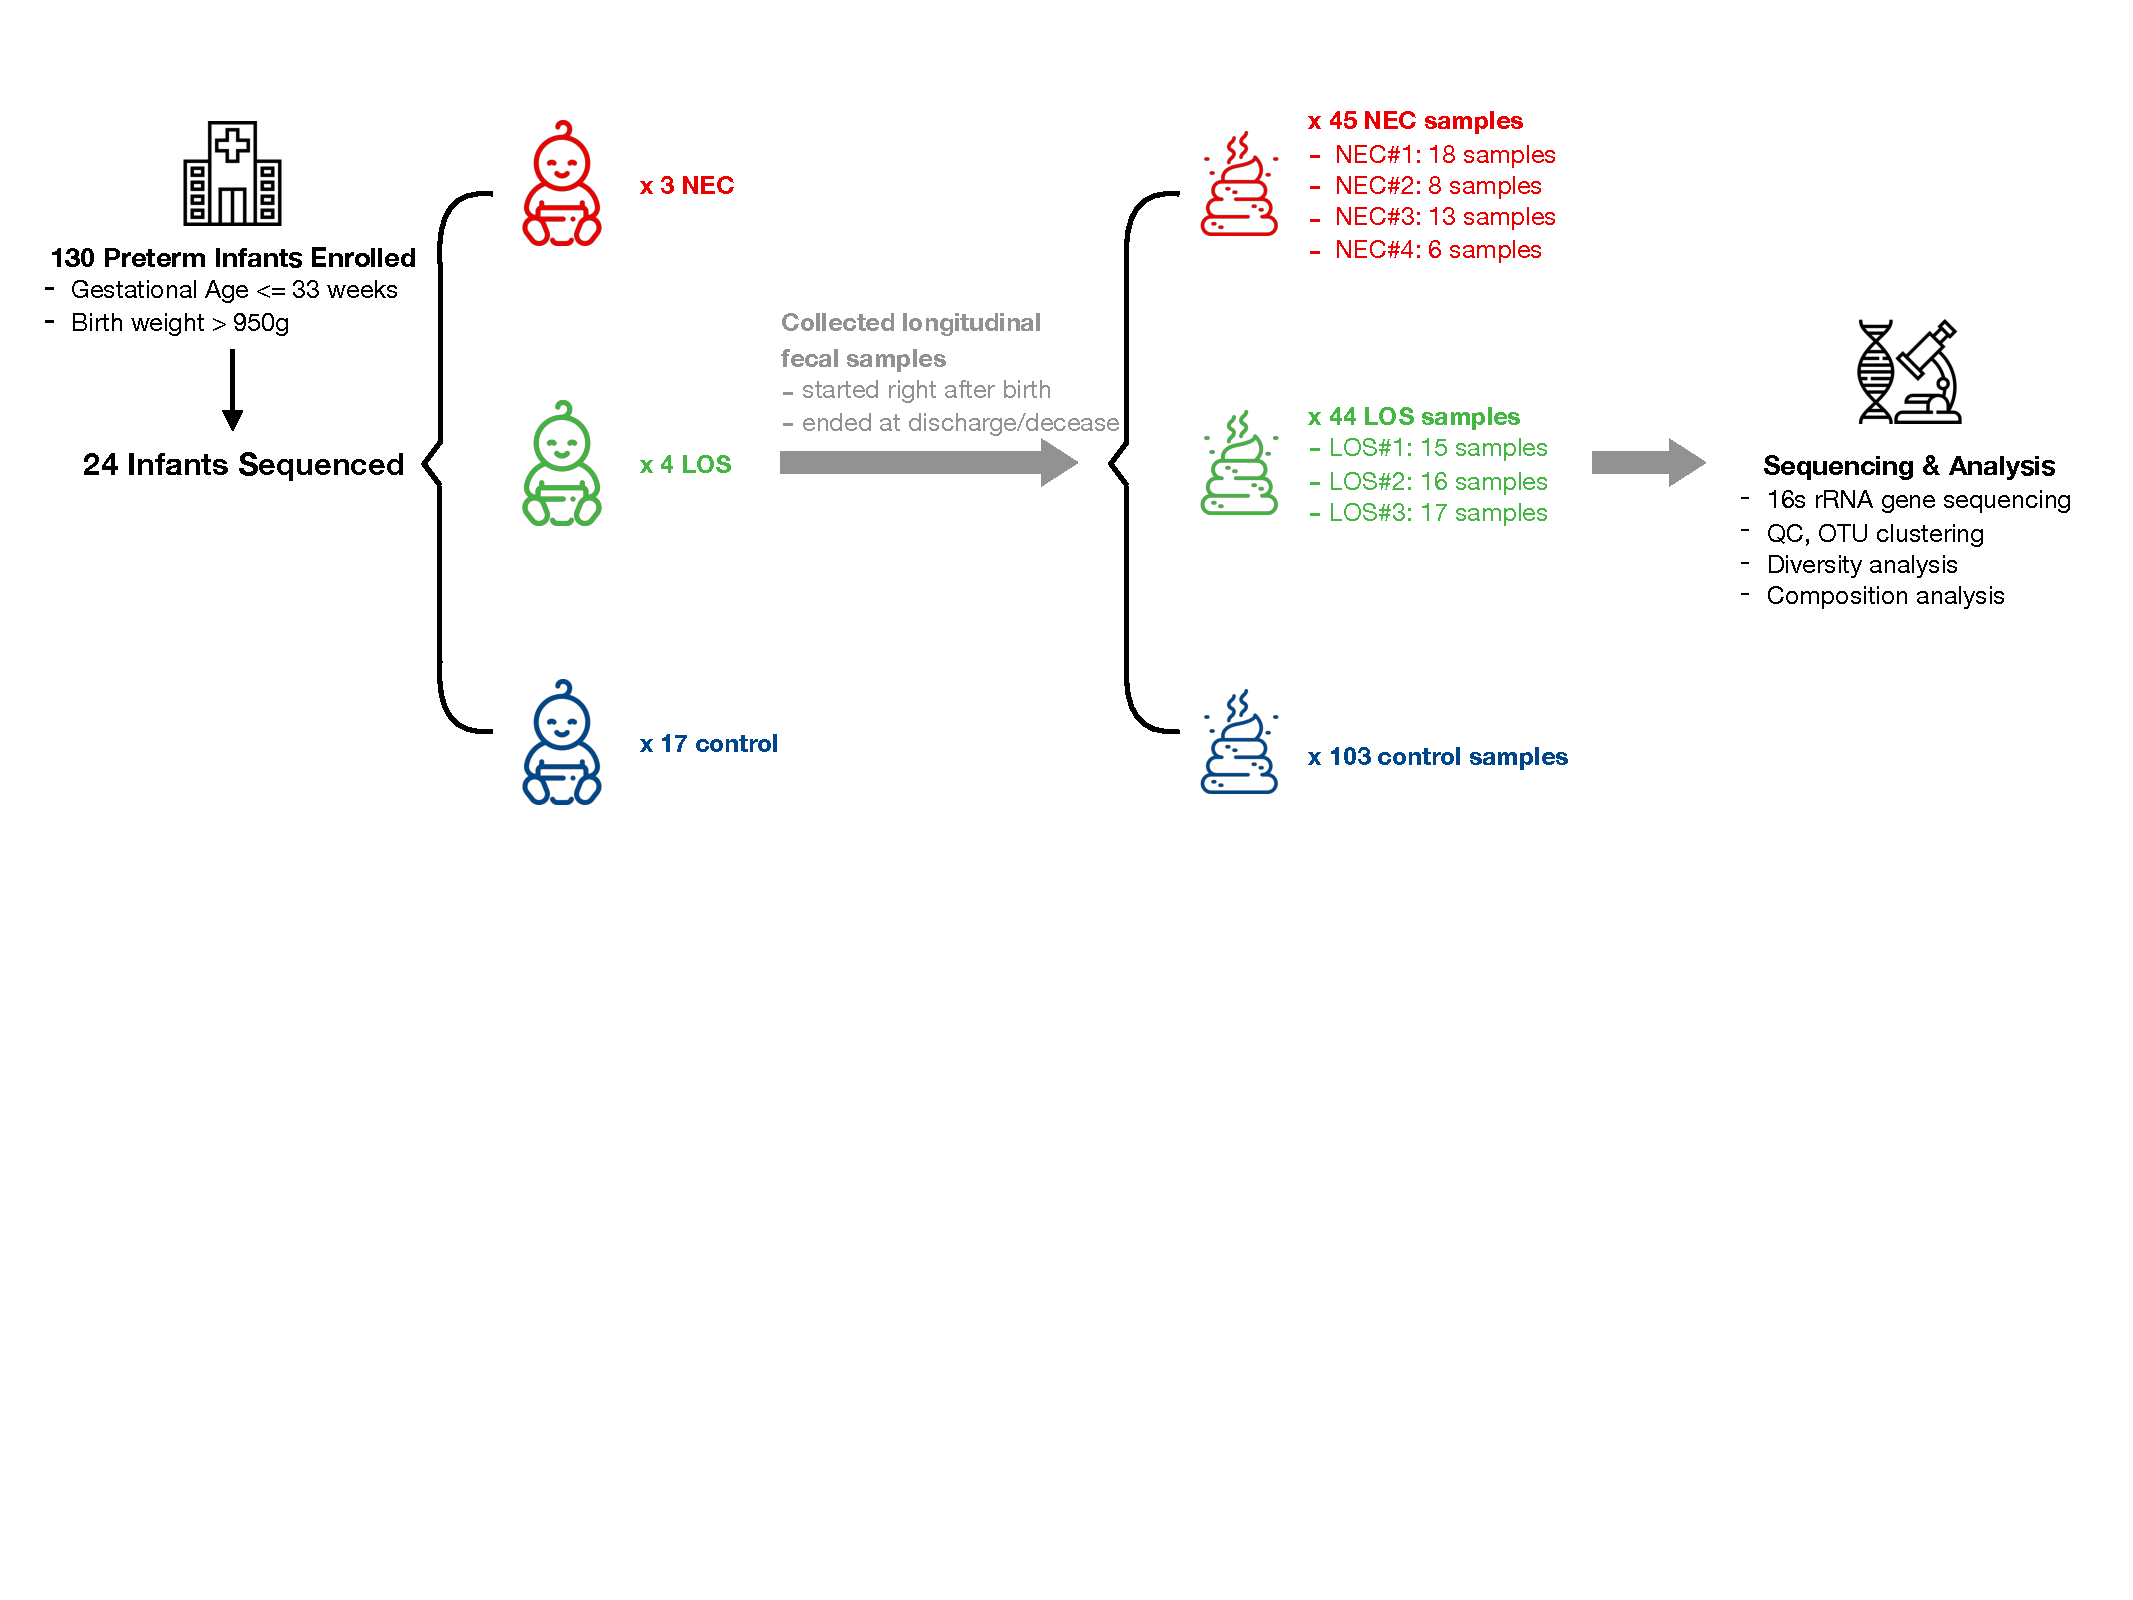
\includegraphics[width=\linewidth]{figure/sheme.pdf}
       \caption{Schematic of Study Design}
       \label{fig:design}
     \end{figure}

     \emph{Fig 1 legend: Schematic of Study Design. Longitudinal fecal samples were collected over from birth to decease or discharge from preterm infants in the NICU. Bacterial diversity and compositions were then characterized.}

  \noindent
   All 24 infants sampled were delivered by cesarean section and fed on infant formula. No infant was prescribed probiotics during hospitalization. There was no significant difference in terms of gestational age(p = 0.074), birth weight(p = 0.11) or gender proportions(p = 0.820) among three groups. The average age at diagnosis for both disease group was 16 days and there was no statistical difference between the groups (p = 0.629) (Table~\ref{tab:demographic}). Therefore, we assigned day 16 until discharge as early disease, day 4-8 as early pre-onset, day 9-15 as late pre-onset interval for the control group.
    \begin{table}[!hpb]
       \centering
       \caption{\label{tab:demographic}Demographic characteristics of Preterm NEC, LOS and control groups.}
      \begin{tabular}{lp{1.8cm}p{1.8cm}p{1.8cm}p{2cm}c}
        \toprule
          & \textbf{NEC (N=3)} & \textbf{LOS (N=4)} & \textbf{Control (N=17)} & \textbf{Statistical Test} & \textit{p value} \\ \midrule
        \textbf{Gestational Age (weeks)} & 29(29-30) & 30(29-31) & 31(28-33) & Kruskal-Wallis test & 0.074 \\
        \textbf{Birth Weight(g)} & 1416.3 (773.4-2149.1) & 1141.7 (633.4-1649.9) & 1527.4 (1391.6-1663.1) & Kruskal-Wallis test & 0.111 \\
        \textbf{Gender} &  &  &  & Fisher's exact test & 0.820 \\
        \multicolumn{1}{r}{Female} & 3(75\%) & 2(67\%) & 9(53\%) &  & \\
        \multicolumn{1}{r}{male} & 1(25\%) & 1(33\%) & 8(47\%) &  & \\
        \textbf{Diagnosis Age(days)} & 16(11-19) & 16(10-22) & — & Wilcoxon rank-sum test & 0.629 \\
        \textbf{Length of Stay(d)} & 54.3 (13.5-95.0) & 60.0 (24.8-95.2) & 32.9 (26.3-39.5) & Kruskal-Wallis test & 0.046 \\
        \textbf{Number of Samples} & 46 & 42 & 103 & — & — \\ \bottomrule
      \end{tabular}
    \end{table}

   \subsection*{Dynamics of Microbiome Diversity in diseases onset and progression}
    \subsubsection*{Microbiome Richness Analysis}
    Furthermore, pairwise comparions between any adjacent two time intervals within the same group(supplementary sobs-time-group!!!!!) didn't show significant alterations and differences in sobs, indicating the minor effect of microbiota richness on the diseases acquisition.

    Overally, all three groups showed similar microbiota richness trend with the observed species (Sobs) decreased significantly from early post-partum period (EPP) to early disease (ED) stage (Fig\ref{fig:sobs-group-time}a. NEC group, p = 0.044; b. LOS group, p = 0.013; c. control group, p \textless 0.01; supplemantary!!! rm-matrix1-sobs, two way RM ANOVA, p \textless 0.0001).  The biggest decrease in richness was between early pre-onset (EPO) to late pre-onset (LPO).  However, the decrease in the disease groups was less significant than the normal group ( NEC group p=0.18, LOS group p=0.066, normal p=0.0004). The Sobs then stabilized from LPO onword with no significant difference between adjacent time intervals.

      \begin{figure}[ht]\centering
        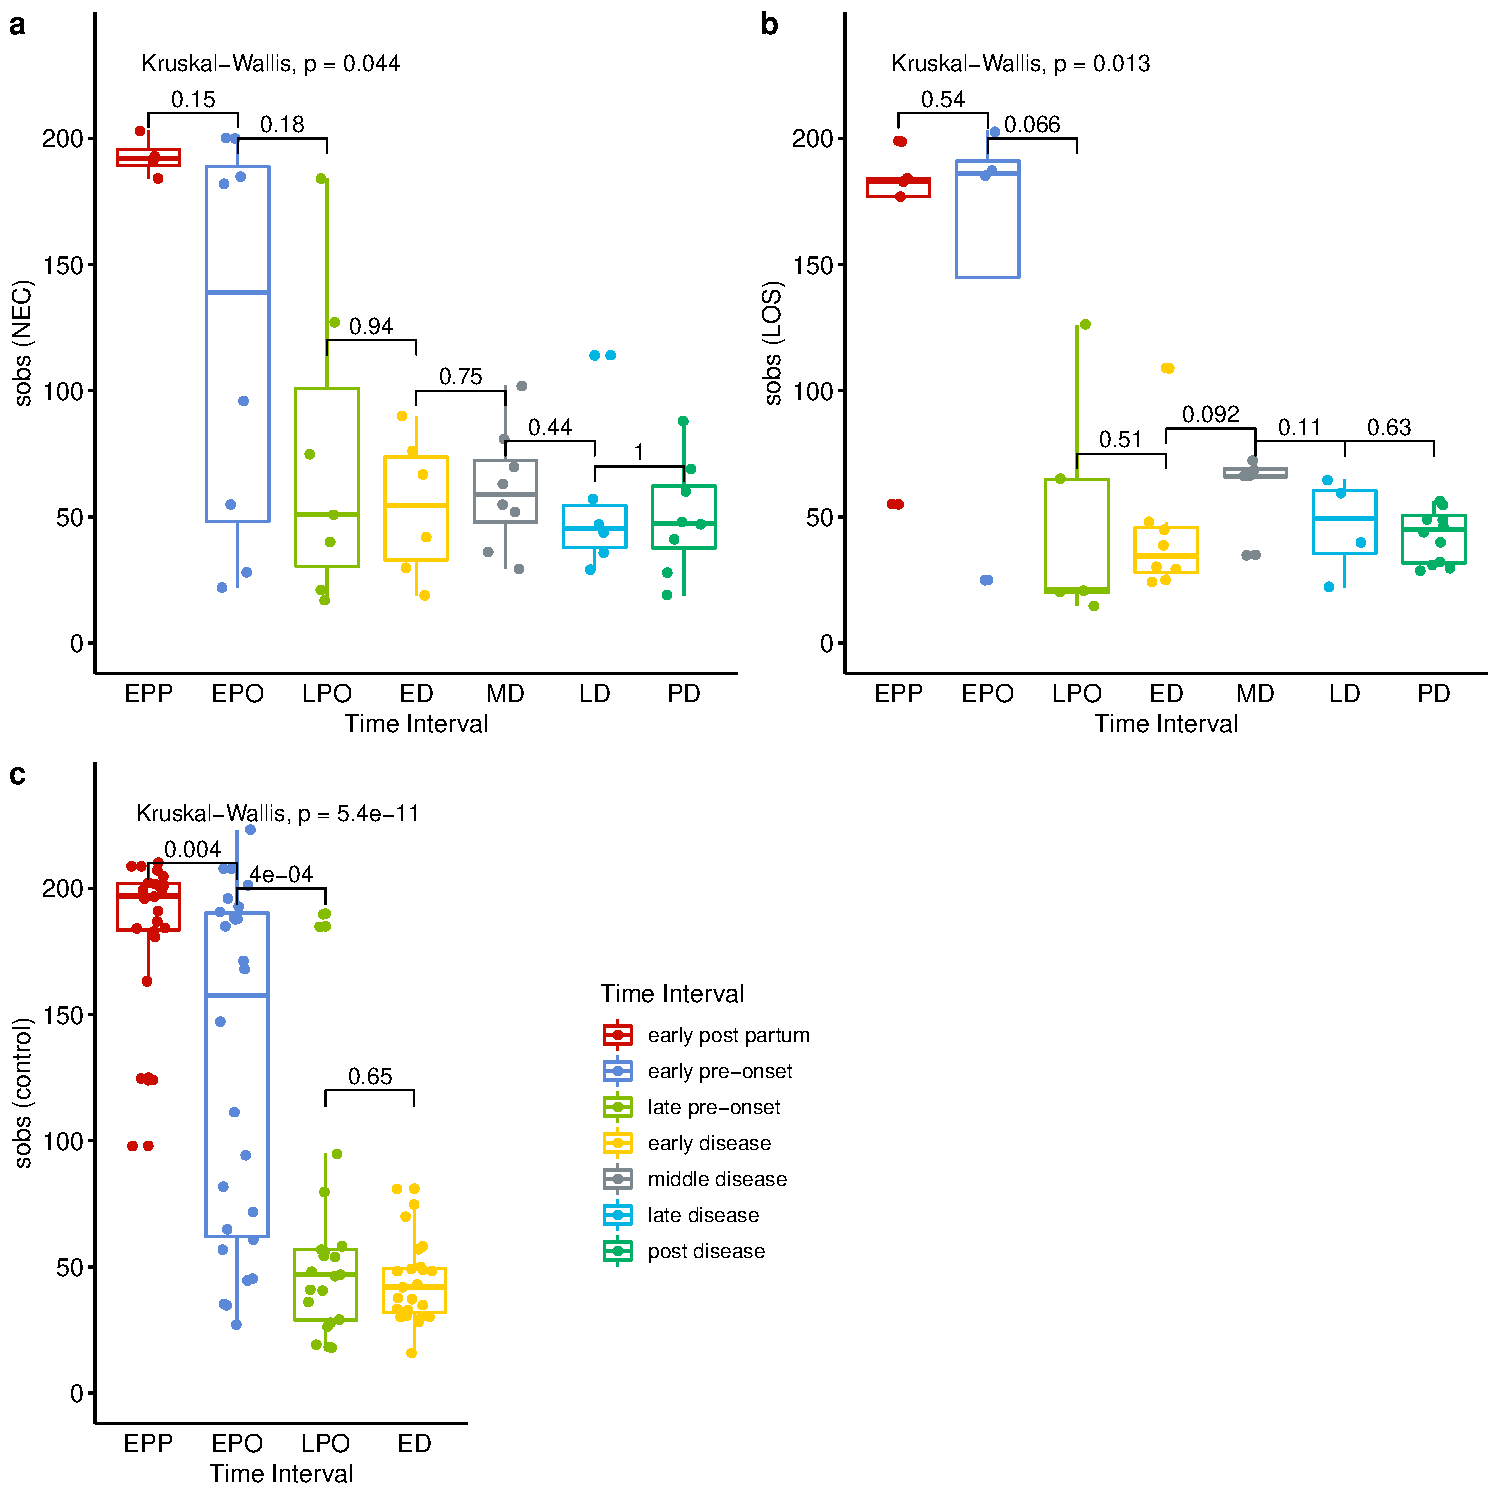
\includegraphics[width=\linewidth]{figure/sobs-group-time.pdf}
        \caption{Post-partum microbiome richness (Sobs) trend in each group}
        \label{fig:sobs-group-time}
      \end{figure}

      \textit{Fig2. Post-partum microbiome richness (Sobs) trend in each group. \\ Shows microbial richness trend in stools from cases and controls (a. NEC group, b. LOS group, c. control group). Horizontal line shows median, box boundaries show 25th and 75th percentiles. Sobs index value of each stool is depicted as one dot. Sobs decreased significantly among three groups from early post-partum to early disease interval(two way RM ANOVA, p <0.01). Timewise comparisons however, shows non-significant trends in bacterial diversity associated with NEC or LOS onset in stools in each group. }

    \subsubsection*{Microbiome Evenness Analysis}
    Similar to microbiota richness, the microbiome evenness represented by shannon diversity indices, decreased from early post-partum (EPP) to early disease (ED)(Fig\ref{fig:shannon-group-time}, supplemantary!!!! rm\_matrix1\_shannon, p \textless <0.0001), the shannon index of the NEC and LOS groups, from the early pre-onset interval to early disease decreased significantly (Fig\ref{fig:shannon-group-time}a.NEC group, early pre-onset = 1.92, early disease = 0.58, p = 0.04, b. LOS group, early pre-onset = 2.47, early disease = 0.47, p = 0.01), while the control group did not show the similar trend (Fig\ref{fig:shannon-group-time}c.control group, early pre-onset = 1.81, early disease =1.00, p = 0.05).
    \begin{figure}[ht]\centering
      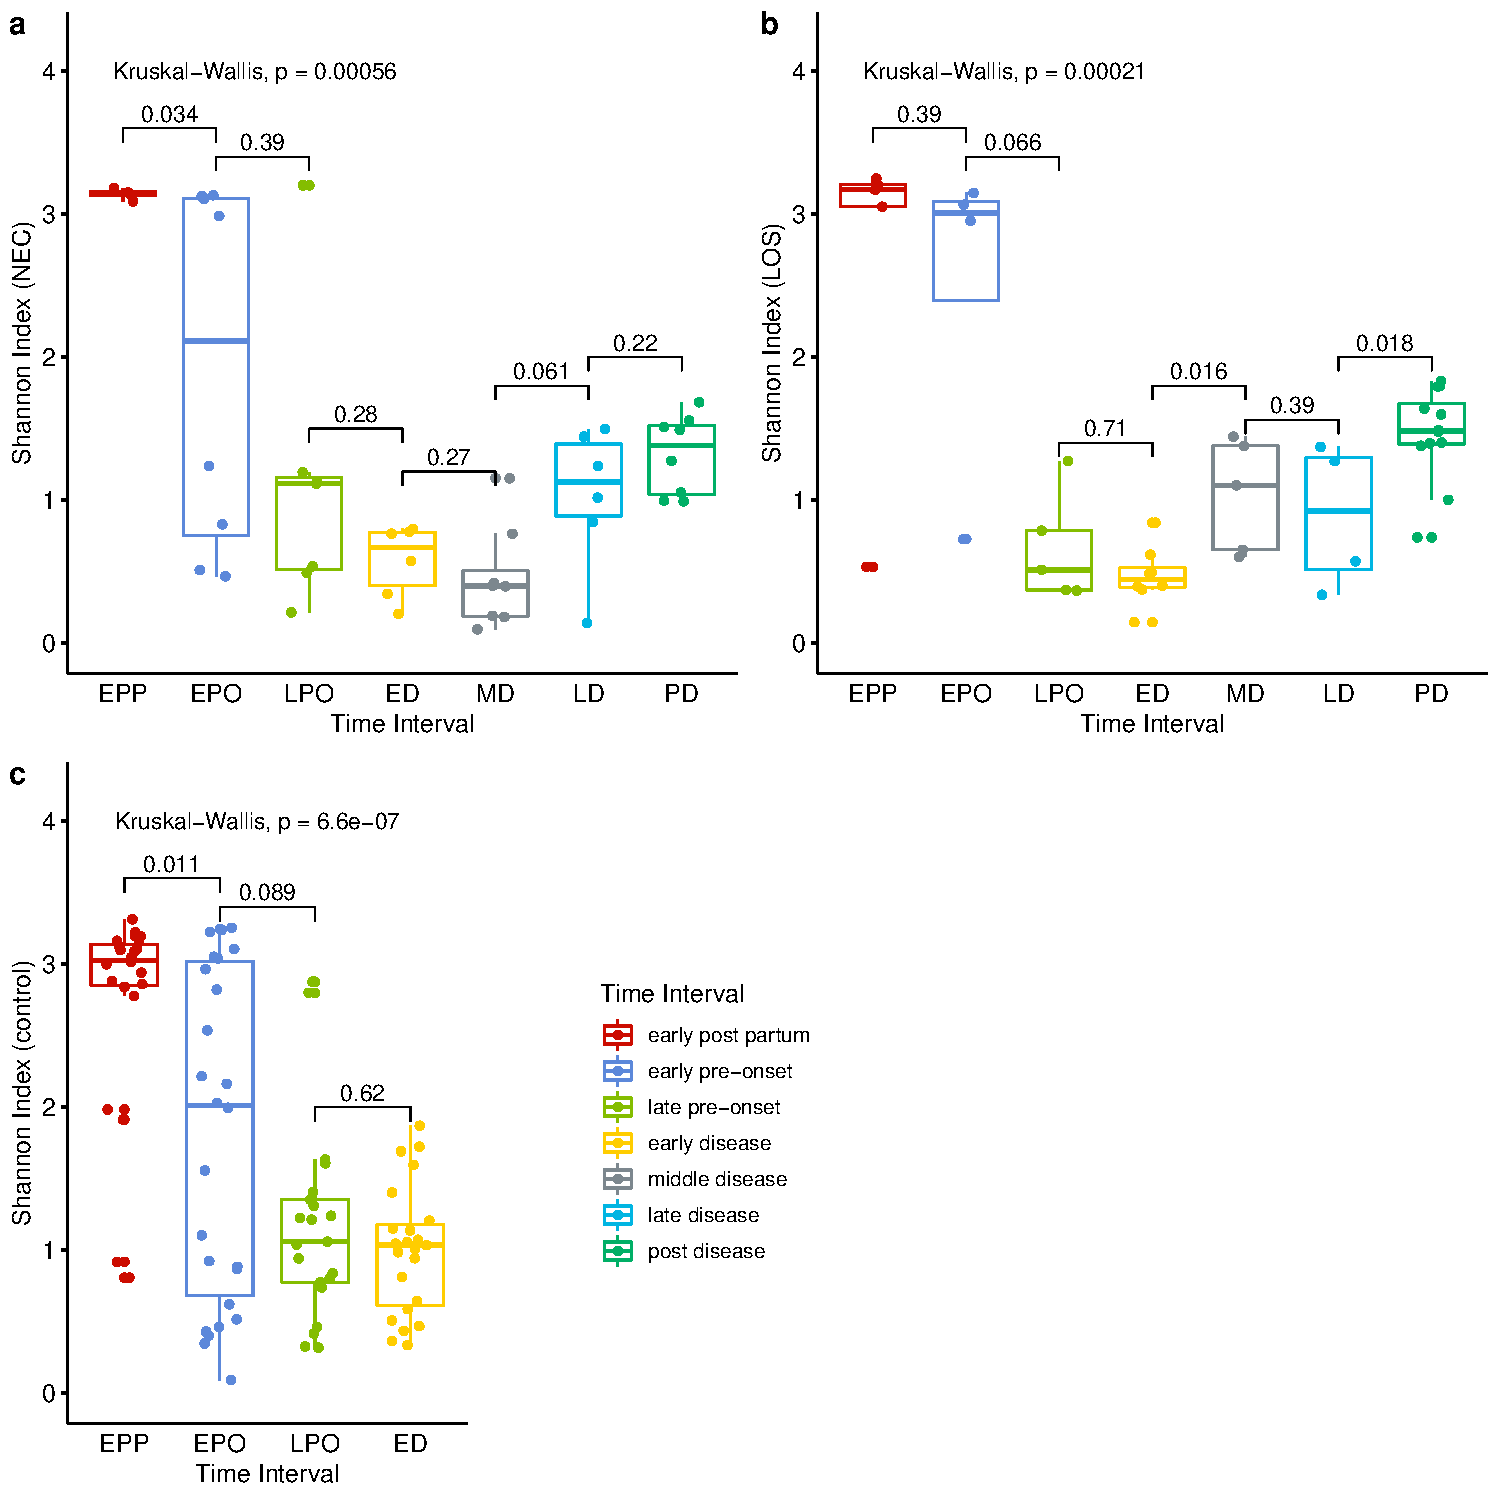
\includegraphics[width=\linewidth]{figure/shannon-group-time.pdf}
      \caption{Post-partum microbiome evenness(shannon diversity index) trend in each group}
      \label{fig:shannon-group-time}
    \end{figure}

    \textit{Fig3. Post-partum microbiome evenness (Shannon) trend in each group. \\ Shows microbial richness trend in stools from cases and controls (a. NEC group, b. LOS group, c. control group). Horizontal line shows median, box boundaries show 25th and 75th percentiles.  Shannon index value of each stool is depicted as one dot. p=0·004 for NEC and p = 0.010 for LOS from early pre-onset to early disease indicating significantly discordant trends in bacterial diversity preceding disease onset. }


    \noindent
    The inter-time-interval comparison among three groups showed significant shannon index divergent during during early pre-onset interval (two way RM ANOVA, p = 0.0017 supplementary!!!) and the early disease stage(Fig\ref{fig:shannon-time-groups}, p = 0.0037), implying the role of microbiota distortion in triggering NEC and LOS. As diseased progressed, two disease groups showed a non-significant difference in community evenness(Fig\ref{fig:shannon-time-groups} facet "middle disease", p = 0.034), indicating a similar community distribution pattern in both NEC and LOS development. Finally, alleviation of both diseases restored the microbiota evenness back to the early pre-onset level respectively (Fig\ref{fig:shannon-group-time} a. NEC, early pre-onset vs. post disease, p = 0.79; b. LOS, early pre-onset vs. post disease, p = 0.16).
    \begin{figure}[ht]\centering
      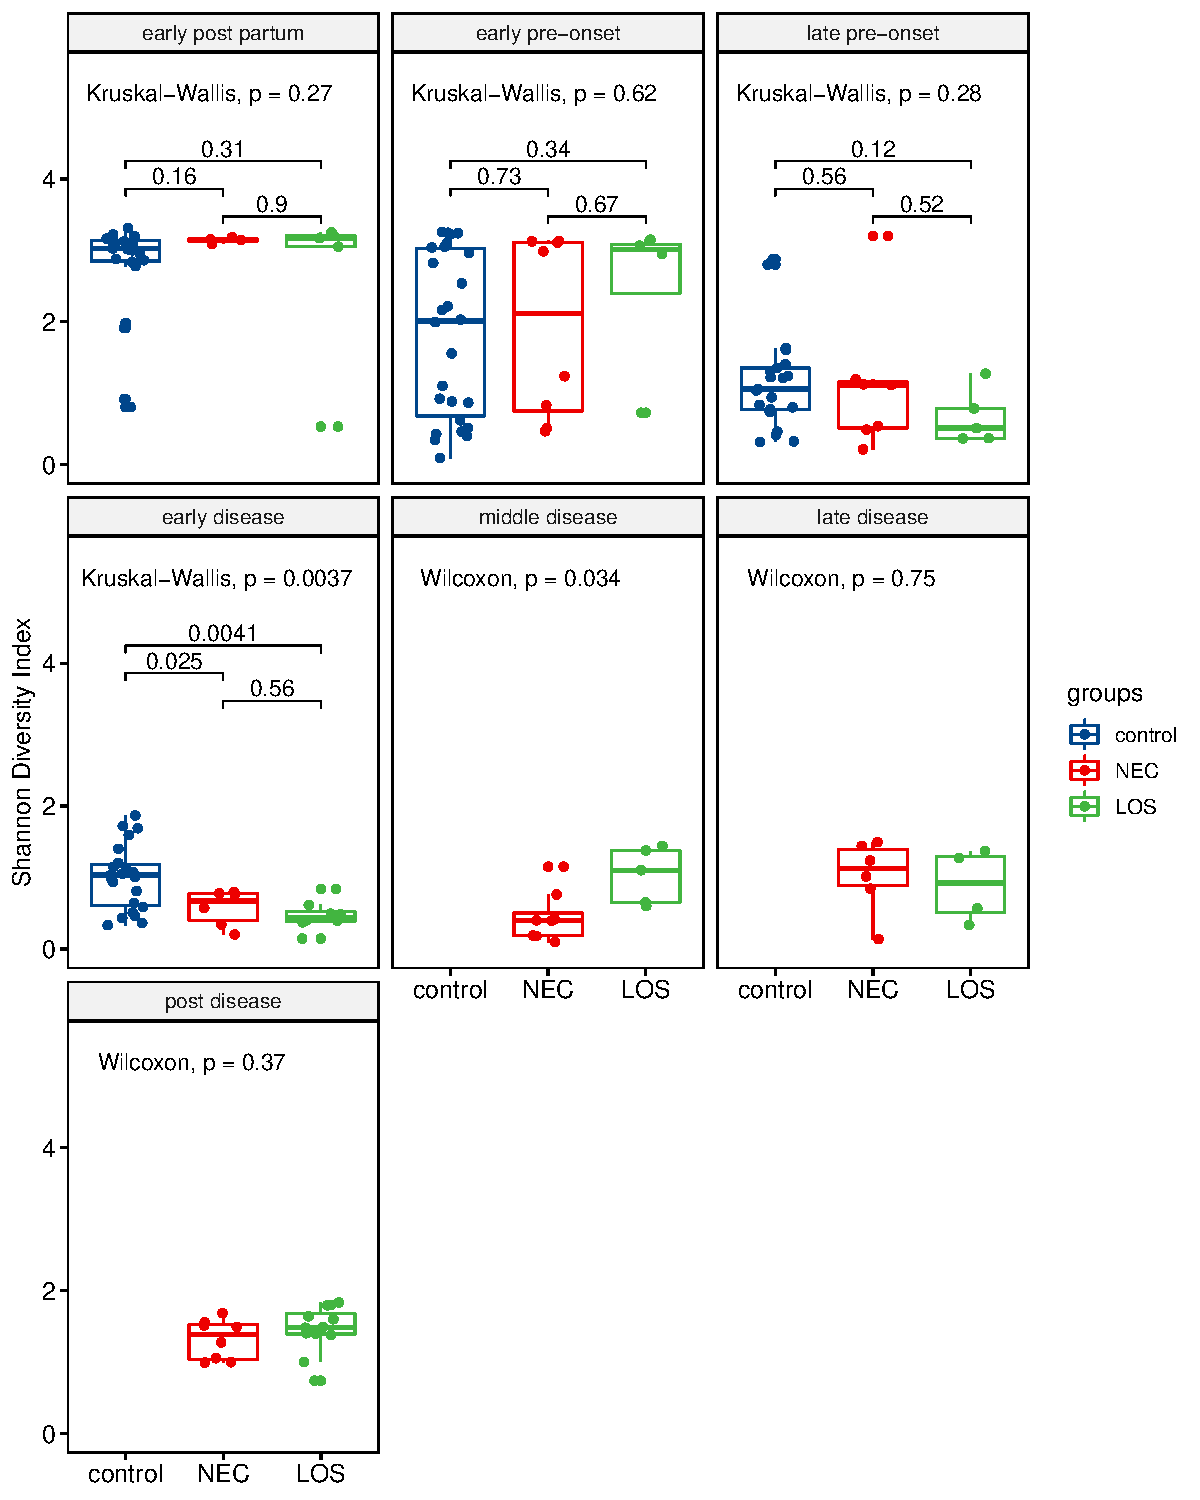
\includegraphics[width=\linewidth]{figure/shannon-time-groups.pdf}
      \caption{Post-partum microbiome evenness(shannon diversity index) trend in each time interval}
      \label{fig:shannon-time-groups}
    \end{figure}
    \textit{Fig4. Post-partum microbiome evenness (Shannon) in each time-interval. \\ Shows microbial richness trend in stools from cases and controls (a. NEC group, b. LOS group, c. control group). Horizontal line shows median, box boundaries show 25th and 75th percentiles.  Shannon index value of each stool is depicted as one dot. p=0·004 for NEC and p = 0.010 for LOS from early pre-onset to early disease indicating significantly discordant trends in bacterial diversity preceding disease onset. }


    \subsubsection*{Kinetics of Microbiome Composition}
    To evaluate time-wise differences in beta-diversity between the microbiomes, we applied Principal Component Analysis (PCoA) to weighted UniFrac distance matrix, considered by timer intervals. During early post-partum interval, beta-diversity among three groups was the lowest with the first principal coordinates accounted for 33.01\%.
    Over time, beta diversity started to drift away from one another from early pre-onset to early disease, with the first principal coordinate accounted for 35.23\% at early pre-onset phase, to 42.32\% in early disease phase((Fig\ref{fig:pcoa})b to d), implicating that the phylogenetic compositions of the case stools already deviated from the control ones before the onset of disease. As disease progress, the phylogenetic dissimilarity between the disease groups further separated and peak at middle disease stage (59.53\%) then came down gradually to 42.8\% at post disease stage (Fig. 5 e to g)  This phylogenetic dissimilarity may suggest  difference in  etiopathology at the pre-onset stage while the differences between the disease group may be a result of different antibiotic regimes for NEC and LOS.
    \begin{figure}[ht]\centering
      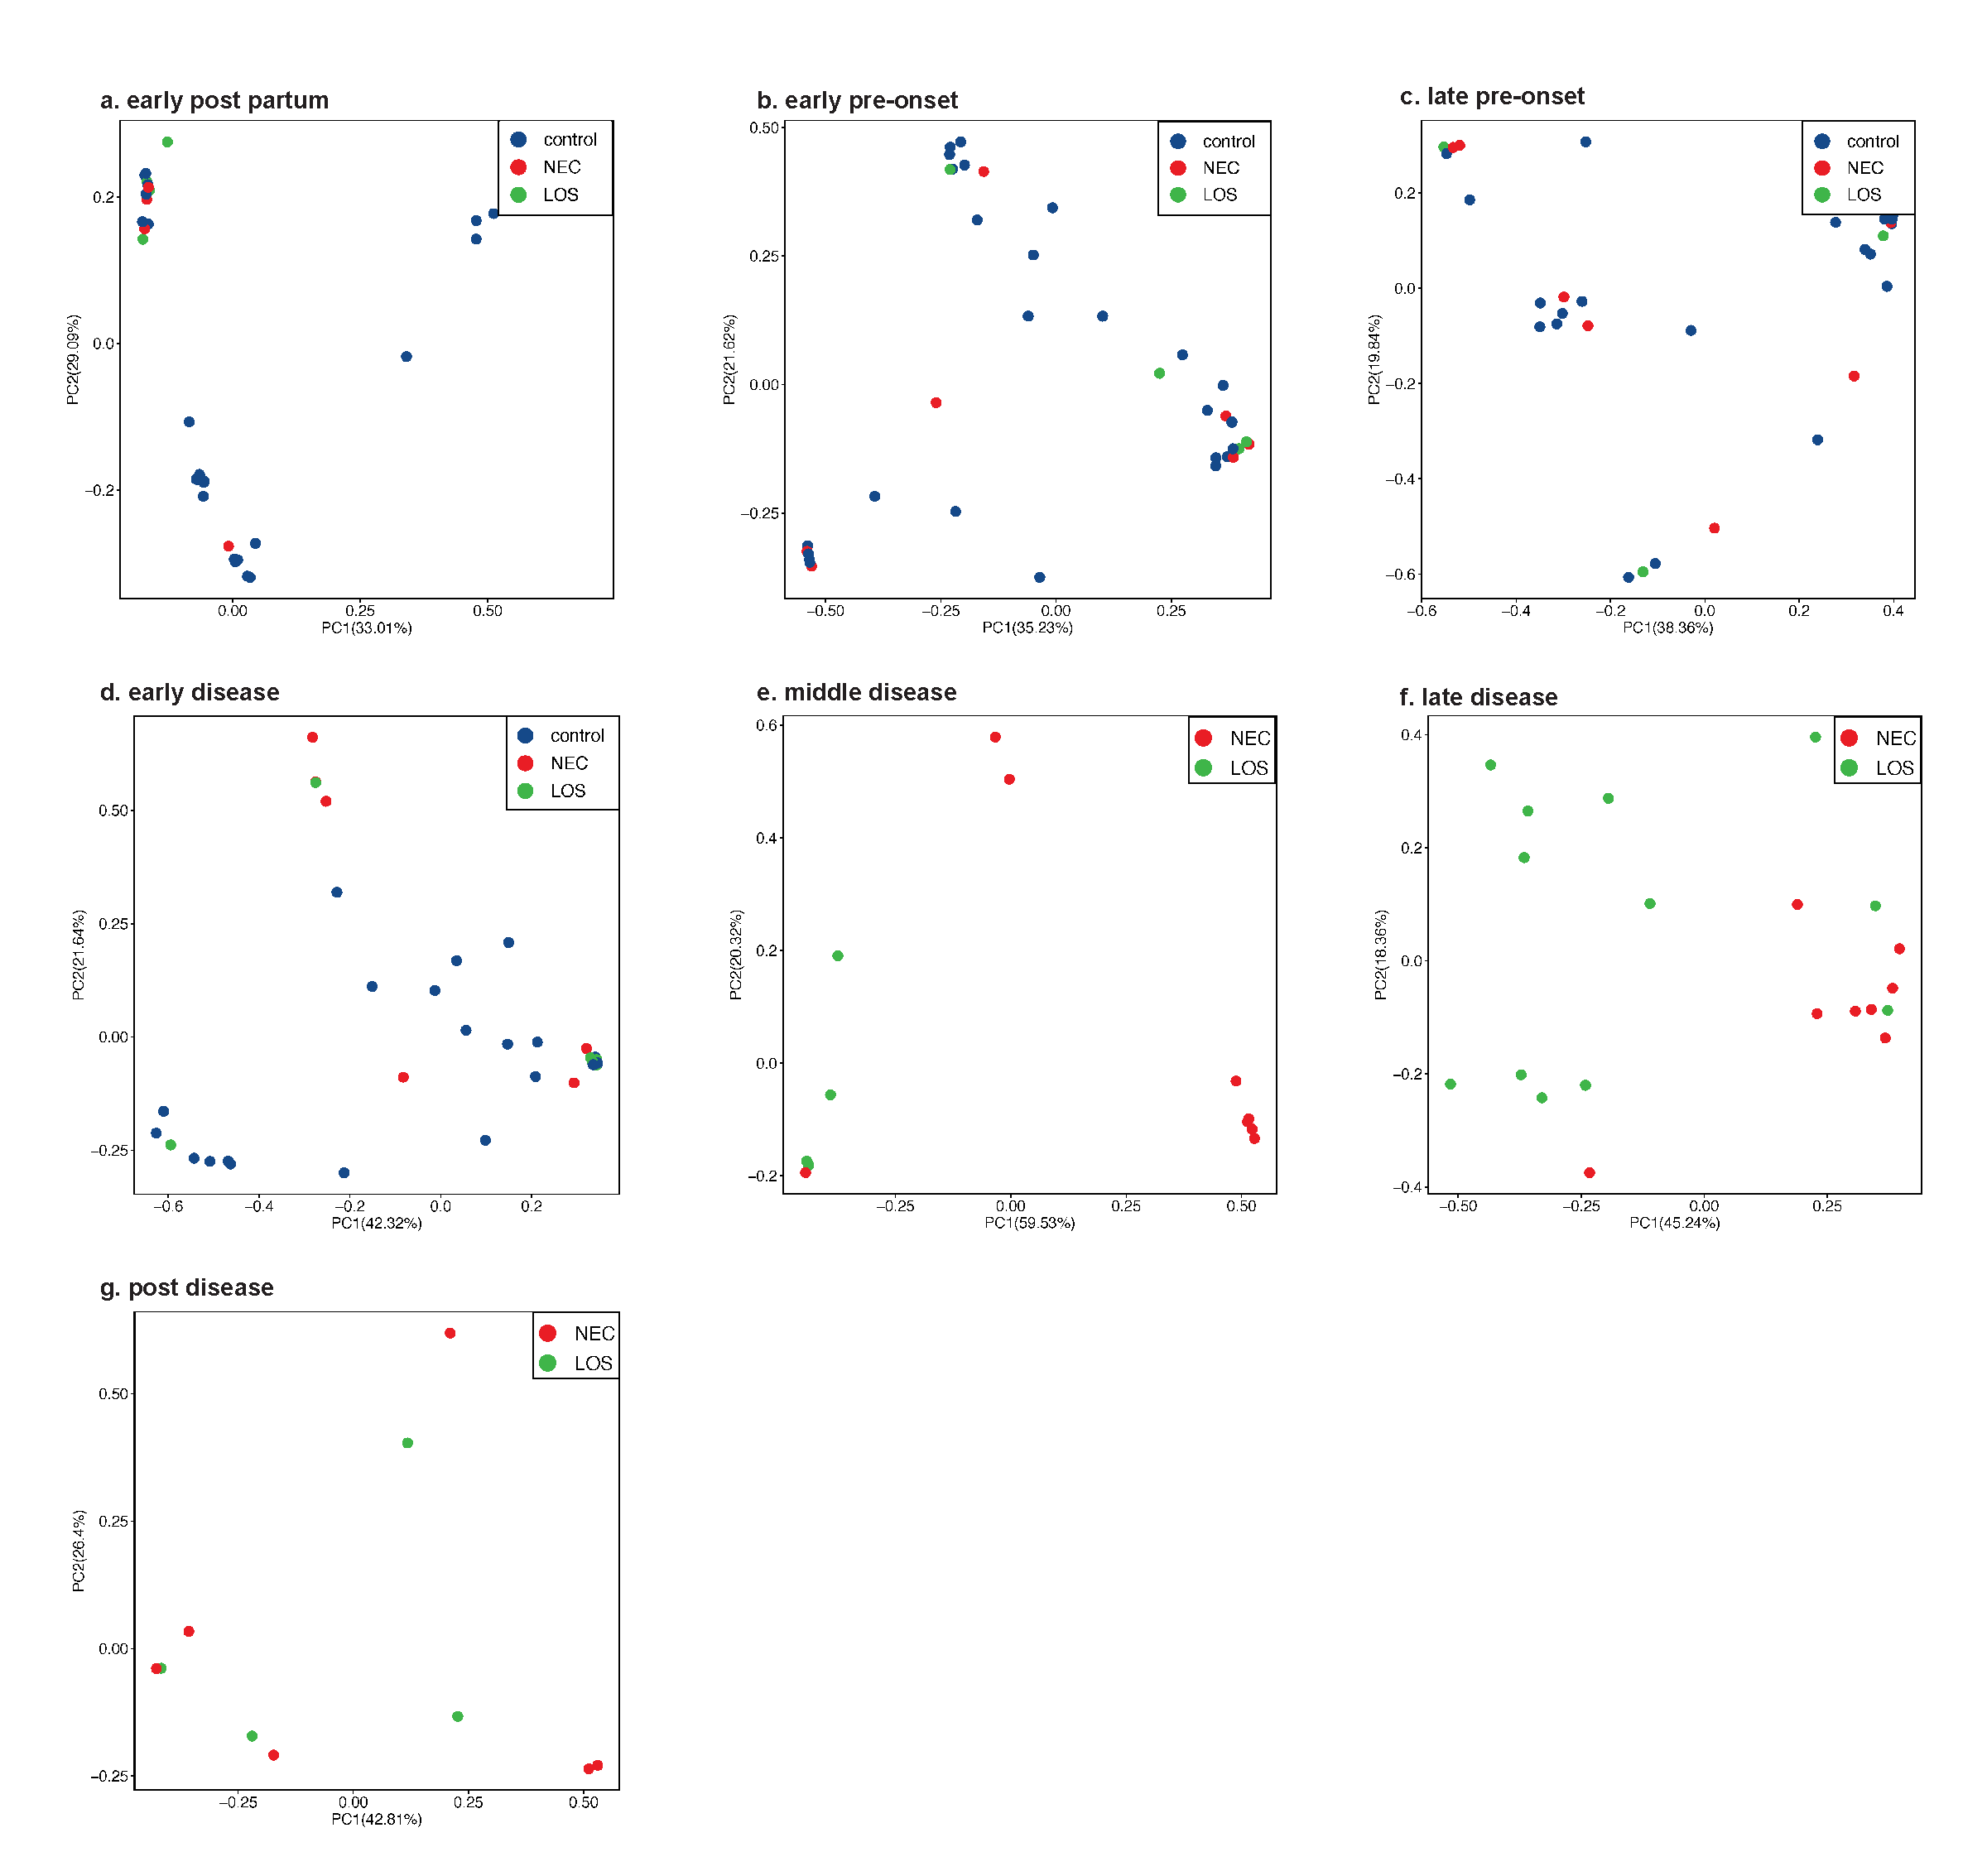
\includegraphics[width=\linewidth]{figure/pcoa_time_group.pdf}
      \caption{Beta Diversity}
      \label{fig:pcoa}
    \end{figure}


    \emph{Fig 5 Principal coordinates analysis ‘PCoA’ plot (beta diversity) demonstrating unweighted UniFrac distance between sample with group points colored for NEC, LOS and control infants. Scatter plot shows principal coordinate 1 (PC1) versus principal coordinate 2 (PC2). Percentages shown are percentages of variation explained by the components. Each dot represents the microbiota of a single sample, and colors reflect the grouping information for that sample. Samples that are clustered closely together are considered to share a larger proportion of the phylogenetic tree in comparison to samples that are more separated. During early post-partum interval, three groups have similar beta diversity. But as approaching disease status beta diversity drifted further away between case groups and the control group.}

  \subsection*{Colonization Trend on Genus Level}
  In the analyses of microbiome alpha(Fig\ref{fig:sobs-group-time}) and beta diversity(Fig\ref{fig:shannon-group-time,fig:shannon-time-groups}), detectable differences was observed among the three groups, especially during transition from LPO to ED stage.  This suggested that the microbiota compositions of the two disease groups and the normal group might be different.  To further investigate if any change in microbiota composition correlate with the onset and progression of NEC and LOS, we tracked the changes in bacteria at genus level during hospitalization.  We filtered the genus of over 10\% relative abundance among all samples and plotted proportion over time.
  \begin{figure}[ht]\centering
    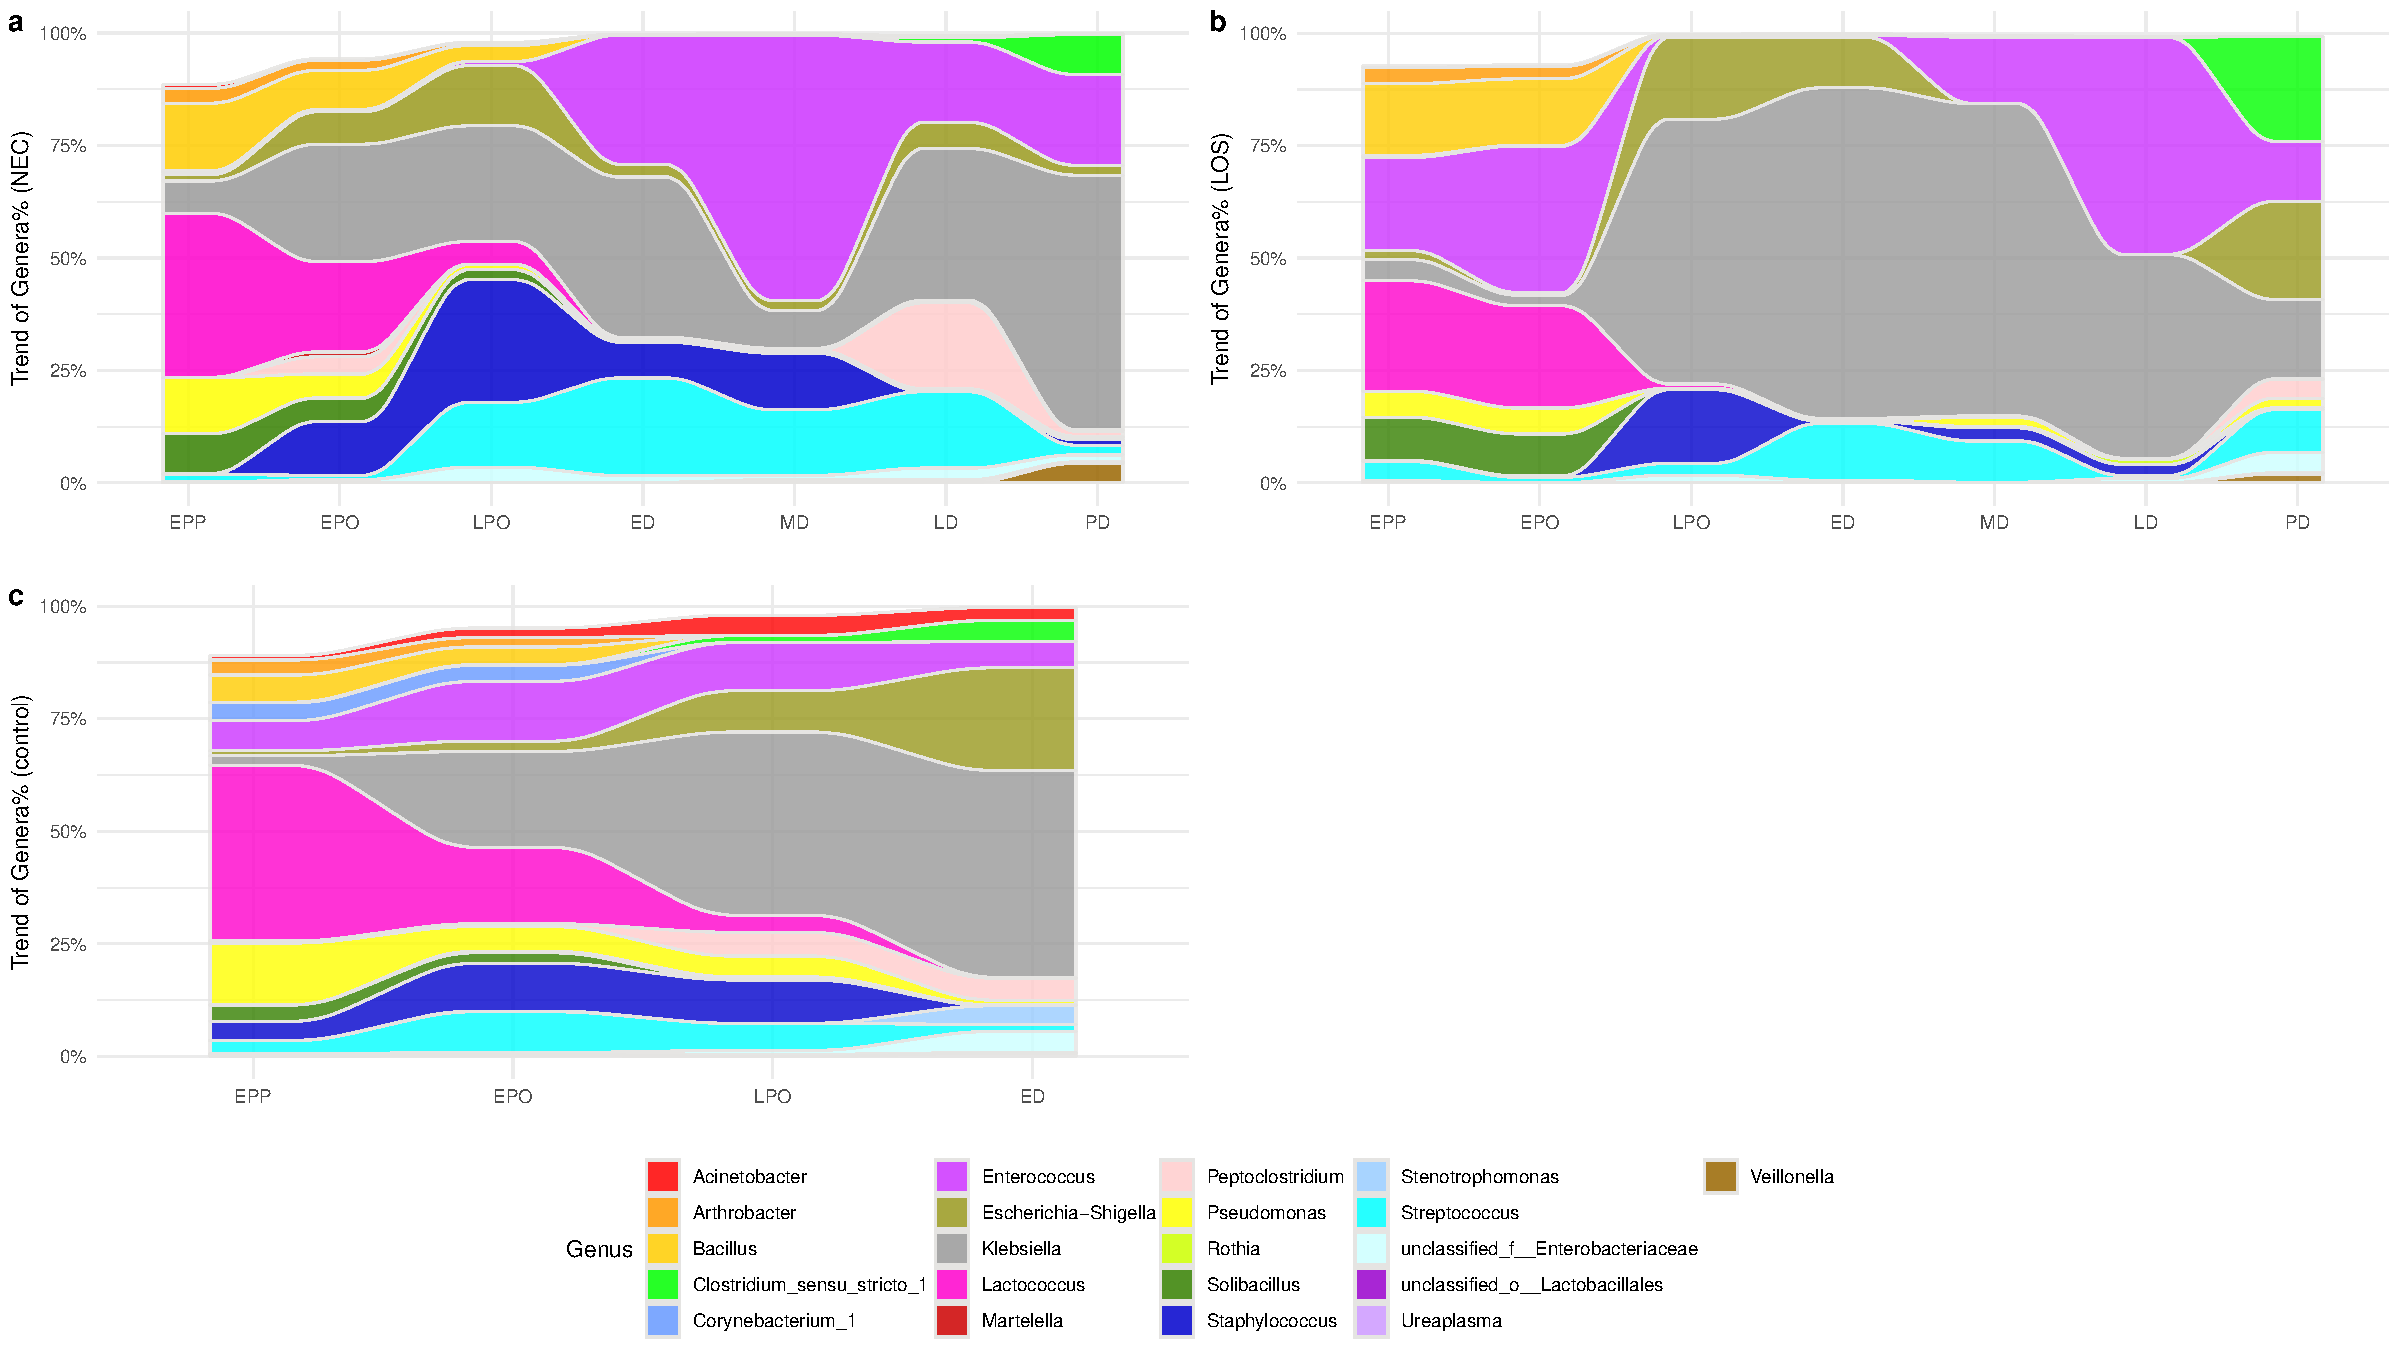
\includegraphics[width=\linewidth]{figure/taxa-time.pdf}
    \caption{Kinetics of Genera Relative Abundance}
    \label{fig:taxa-time}
  \end{figure}

%Bar graph depicting the relative abundance of most commonly encountered bacterial phyla between FT, ELBW and BPD infants.

  \noindent
  Before disease onset, ZIBR model showed significant time-by-NEC and time-by-LOS interaction factors for the progression over time of Bacillus and Solibacillus. At early post-partum stage, all three groups were dominated by Lactococcus, Bacillus and Pseudomonas. However, a rapid decline in was observed in both disease groups showed significantly higher Bacillus(p = 0.032) and lower Solibacillus(p = 0.047) relative to control samples(ZIBR table cited). Furthermore, both case groups experienced a rapid \textit{Bacillus} decline when approaching disease stages(NEC from 15.053\% in early post-partum to 0.011\% in early disease interval; LOS from 15.967\% in in early post-partum to 0.002\% in early disease interval). %这一段要再改

  \noindent
  For NEC samples, \textit{Enterococcus} increased significantly from 0.009\% in late pre-onset phase, to 28.801\% in early disease and 58.959\% in middle disease interval (p = 0.032). Meanwhile, after its transient boost in late pre-onset interval(27.231\%), Staphylococcus had been constantly presented (12.571\%) until late disease interval of NEC. Relative to control samples(6.010\%), NEC samples showed higher Streptococcus(14.439\%, p = 0.023) starting from late pre-onset stage to late disease stage. Peptoclostridium increased during late disease stage(\#diarrhea!!)(Fig\ref{fig:taxa-time}a).

  \noindent
  For LOS patients, a significant outburst of Klebsiella (EPP: 4.7\%, EPO: 2.376\%, LPO: 58.902\%) with diminishment of other genus were characterized prior to the disease onset. Later on, Klebsiella aggressively dominated the intestine throughout the whole course of disease(ED: 73.529\%, MD: 69.506\%, LD: 45.333\%). By contrast, Escherichia-Shigella, which might well be impacted by advanced antibiotics including Meropenem, was absent from late pre-onset to early disease interval(0.005\%, p = 0.026 and 0.003\%, p = 0.045, respectively), restored until middle disease interval(14.762\%, p = 0.042) and became the second abundant genera dominating the intestine in late disease(48.336\%, p = 0.262)(Fig\ref{fig:taxa-time}b)

%%%%%%%%%%%%%%%%%%%%%%%%%%%%%% DISCUSSION %%%%%%%%%%%%%%%%%%%%%%%%%%%%%
\section*{Discussion}
% Both necrotizing enterocolitis and late onset sepsis burden china birthrate, in both the developed and developing world.


With a prospective study design, we investigated the longitudinal microbiome diversity and composition, from the Chinese preterm infants who subsequently developed necrotizing enterocolitis or late-onset sepsis. The main findings were that among case stools, the overall microbiota diversity was reduced and specific compositional characteristics of the microbiota was associated with potentially pathogenic genus, such as \textit{Enterococcus}, \textit{Staphylococcus}, \textit{Peptoclostridium} and \textit{Streptococcus}.

Inter-sample diversity decrease postpartum,

compare to control, phylogenetic dissimilarity emerged preceding disease
consistent with previous studies. continuous

oppotunistic
initially


\noindent
Both case groups and control group showed decrease in richness and evenness after birth. In previous studies Several studies suggested a reduction in microbiota community diversity Community richness

1. alpha  1.1 evenness minor rols 1.2 richness dicrease during  (corresponding 4~7 dol) may precede diseases, less diversified <-> s/s? \# consistent with the hypothesis that dysbiosis precedes this severe event.
2. beta
3. over/underrepresenting of certain genus
4. Microbiome optimization -- a novel strategy

%The anaerobic, milk-degrading bifidobacteria were largely absent, even in preterm infants with access to breastmilk, possibly due to a lack of exposure to microbes from family members in the sterile hospital environment, along with antibiotics.

\noindent
Our study was limited to 1 hospital in one specific geographical region in China and so could not be generalized to a larger population. Our results, however, showed the needs of an exceptionally larger, more heterogenous study population to confirm our findings
Our study has its limitations. We acknowledge that the sample size is limited since this study is single-center-based and the incidence of both diseases are relatively low: among the 1148 preterm infants admitted within July 2013 to December 2014, only five developed NEC. The resultant overfitting possibility inevitably rose up, which became the pitfall in understanding the true microbiota patterns of NEC and LOS. Our results, however, showed the needs of an exceptionally larger, more heterogenous study population and longer follow ups, to draw a more meaningful and solid conclusion within the non-western population.

\section*{Conclusions}
To our knowledge, our study is the first to report intestinal microbiota of Chinese preterm infants using 16s rRNA gene NGS data. Intestinal microbiota diversity reduction and phylogenetic dissimilarity away from healthy infants over time is associated with both NEC and LOS onset. Over-growth  of potentially pathogenic genera were recognized, i.e. \textit{Enterococcus}, \textit{Streptococcus} and \textit{Peptoclostridium} in NEC cases; \textit{Klebsiella} in LOS cases. Our results is a starting point for further studying of microbial factors involved in preterm-associated complications within China range. A better understanding of microbial risk signatures in longitudinal microbial community assembly during early life, including its colonization mechanism and interaction with intestinal immunological responses, would assist in better understanding the etiology and assist in development of alternative biomarkers for early diagnosis and facilitate novel prevention and treatment strategies, to protect predisposed preterm infants in Chinese population.

\section*{Acknowledgments}
We sincerely thank all the patients and their family  in  supporting  this study. We extend our thanks to the medical and research staffs of the Shanghai Children’s Medical Center.  We also thank Ka Ming Pang and Arin Nam for critical review of this manuscript.

%microbiota development in infancy, sequence effect, Conversely, adequate maturation of the gut microbiome in this period may protect these pre-disposed children.
%increase vulnerability
%kinetics
% supplementary: otu

%"#00468BB2" "#ED0000B2" "#42B540B2"






\bibliography{manu}

\end{document}
